\indent
In the last decades, we witnessed a growing demand for performing large-scale
computations, such as protein folding, fluid dynamics, weather and market prediction, or production process optimization.
The scale of such computations exceeds abilities of a single computer, hence they need to be performed on large sets of machines that cooperate over an interconnecting network.
Owning and maintaining such large-scale computing infrastructure is often impractical and expensive, and parties look for alternative ways to perform computations.
In comparison, outsourcing computations provides a wide range~of~benefits.
First of all, it mitigates the costs of infrastructure management and maintenance.
This is crucial especially for computational tasks that arise occasionally, such as high-quality rendering, computer verification of products with long development time or analysis of human-harvested data.
Second, such an approach dismisses the need to foresee the appropriate demand for resources.
If such demand increases unexpectedly, it can be immediately provided without physical extension of the infrastructure.
This led to a shift of computations to large-scale remote facilities that contain computing machines with their support infrastructure, the so-called \emph{data centers}.
Performing computations in these external data centers provides the impression of unlimited computational power on demand, and is called the \emph{cloud computing}.

The demand for outsourcing computations to the cloud created a whole market for such services.
Modern suppliers of processing power such as Microsoft Azure \cite{url-azure}, Amazon Web Services \cite{url-amazon-ec2} or Google Compute Engine \cite{url-gce} provide convenient on-demand computational power while hiding most of the details concerning resource management.
Processing capabilities are quickly and conveniently accessible to every interested party.

Computational tasks require multiple types of resources to complete: CPU time, memory, I/O operations and network bandwidth.
Often the demand for these resources varies in time and is unpredictable.
For this reason, a data center that performs just one task at the time would waste resources.
In contrast, the co-existence of multiple tasks in the data center allows to~compensate for the variable demand for resources by resource-aware scheduling.
Such techniques are especially useful in (but not limited to) computationally-intensive applications, where the response time is not the primary concern.

\pagebreak

\medskip
The first part of this thesis assumes the perspective of a data center owner, who wants to~use owned resources in an efficient manner.
For example, the processing speed can be scaled down to save energy, memory can be shared or distributed, and cooperating processes can be migrated closer to each other in the network to save bandwidth.
In the first part of this thesis, we focus on the~last aspect and we show how it leads to
\emph{efficient usage of an interconnecting network} in a data center.
Optimization of this resource is critical for performing efficient large-scale computations, as these involve multiple machines that cooperate over the network.
To this end, we will make use of a~sophisticated control system, called \emph{virtualization}.

\medskip

In the second part of this thesis, we shift our attention away from the optimization of data center network and focus on fundamental aspects of data transmission in the modern Internet.
The transmitted data is split into portions called packets, which are sent independently, and the task of relaying a packet to its destination, called \emph{packet forwarding}, is performed~by network devices called \emph{routers}.
A~single network is usually connected with multiple adjacent networks, and at each intermediate network, a bordering router needs to determine the next router on~the~way of the packet.
To this end, such device directs packets based on the set of its forwarding rules, each corresponding to some network.
The number of forwarding rules stored in core Internet routers is almost as numerous as the total number of networks, which leads to~enormous forwarding tables to manage.

The second part of this thesis assumes the perspective of an Internet Service Provider (ISP) that owns and maintains the connecting physical infrastructure, such as routers.
Typically, routers located near the core of the Internet, e.g., in top-tier networks owned by large ISP, store a sizeable number of forwarding rules, and this number continues to grow with the size of~the~Internet.
As the size of forwarding tables grows, it inevitably \emph{exceeds the available memory of~the~router}.
One of the goals of the ISP is to utilize existing devices in the most efficient way and to delay the need for an upgrade.
The obvious but expensive solution is~to~provide additional memory for the device.
We focus on an alternative approach, where the router continues to~operate with insufficient memory to store the whole forwarding table.
In~this approach, it is important to preserve the correctness and efficiency of packet forwarding: both are crucial in~minimizing data transfer latency and maximizing the throughput.


\section{Machine Virtualization in Data Centers}
%\sectionmark{Data Center Scenario}
\label{sec:intro-machine-virtualization}

To use the data center's interconnecting network efficiently, cooperating computational tasks should be placed close to each other and close to the data they process.
Algorithmic techniques presented in the first part of this thesis rely upon logical isolation of a computation from the~physical machine that performs the computation.
This gives a~possibility to manage the~physical placement of a computation in a way that is transparent to the computation.
A~particular piece of technology that provides the flexibility in placement of computations is~\emph{virtualization}.

Virtualization provides an abstraction layer, called the \emph{virtual machine}, for the underlying hardware of a computer system.
Virtual machine mimics the functionality of the physical hardware so closely that it can be used as an environment for a complete operating system.
Such operating system, running on a virtual machine is called the \emph{guest
operating system}. It operates in addition to the \emph{host operating
system}, which runs directly on the physical hardware. 
In a data center, the main purpose of virtualization is to provide a complete and non-restricted environment for the client that is isolated from the management software and other clients' tasks.
The guest operating system is restricted to the virtualized environment: it has the perspective of housing a whole computer system.


\subsection{Machine Migration}

Besides providing an abstraction layer, mature virtualization solutions suited for data centers such as Xen
\cite{url-xen}, KVM \cite{url-kvm}, Hyper-V \cite{url-hyperv}, VMware ESXi
\cite{url-vmware}, provide several control features.
In particular, absolute control over the underlying virtual hardware allows to suspend and resume the execution of the guest operating system at will.
Such functionality provides building blocks for the feature of \emph{migration}, which transfers the complete virtual machine to~a~different physical machine.
This is possible without shutting down the guest operating system, and hence it provides a powerful resource management tool that is transparent to clients.

Distributed cloud applications, including batch processing
applications such as MapReduce, streaming applications such as Apache Flink or
Apache Spark, and scale-out databases and key-value stores such as Cassandra,
generate a~significant amount of network traffic and a~considerable fraction
of their runtime is due to network activity~\cite{MogPop12}. For example,
traces of jobs from a Facebook data center reveal that network transfers on
average account for 33\% of the execution time~\cite{orchestra}. In such
applications, it is desirable that frequently communicating virtual machines
are \emph{collocated}, i.e., mapped to the same physical server: 
communication across the network (i.e., inter-server communication) induces
network load and latency. However, migrating virtual machines between servers
also comes at a price: the state transfer is bandwidth intensive, and may even
lead to short service interruptions. Therefore the goal is to design online
algorithms that find a good trade-off between the inter-server communication
cost and the migration cost.
%
%Such mechanisms play an~important role in load balancing in the data center and allow for sophisticated optimizations such as \emph{reducing network distance between communicating virtual machines}.
%In this thesis, we focus on migration capabilities provided by modern virtualization technologies used for efficient usage of important resource in the data center --- the network bandwidth.
The problem central to the first part of this thesis is stated as follows:

\begin{center}
  \emph{How to assign virtual machines to physical machines to optimize network
  usage?}
\end{center}
We elaborate more in the subsequent subsection.

\subsection{Virtual Network Embedding}
\label{sec:virt_net_emb}

The computing power of a single virtual machine is usually insufficient for the client, as~the~resources of a~virtual machine are limited by resources available to its host.
Therefore, data centers provide their resources as a sizeable set of virtual machines connected by a network.
Collectively, the virtual machines with their interconnecting network are called a~\emph{virtual network}, where the cooperating virtual machines are referred to as \emph{nodes} of a virtual network.
To~guarantee a certain quality of service (\emph{QoS}) for a multitude of co-existing virtual networks, up-front bandwidth reservations are required.
However, the generality of performed calculations results in an unpredictability of communication patterns and poses a challenge in the optimization of bandwidth reservations.
In this thesis, we provide algorithms for an efficient management of~network reservations without any assumptions about communication patterns.

To measure the quality of resource management strategy, in Chapter~\ref{ch:static-mapping} and Chapter~\ref{ch:dynamic-mapping} we state formal optimization problems; for now, we only briefly sketch it.
Physical components of a data center are modeled as a~graph called a \emph{substrate network}, in which vertices correspond to physical machines, and edges correspond to an interconnecting network.
A communication cost between a pair of physical machines is proportional to edge-distance in substrate network (the~number of~\emph{hops} in the substrate network).
A communication pattern among virtual machines is~also modeled as a graph, called a \emph{communication graph}.
In such settings, the communication among virtual machines running on certain physical machines can be viewed as a~\emph{graph embedding} of the communication graph into a substrate network~\cite{gupta2001provisioning}.
The main objective is to find an~embedding that locates closely the virtual machines that communicate often.

In this thesis, we study substrate networks in the form of a tree, which closely models the~popular Fat-Tree topology~\cite{fat-trees}.
In this tree topology, only leaves can host virtual machines, and the~sole role of intermediate tree nodes is to transmit data between leaves, see Figure~\ref{fig:tree-topology}.


\begin{figure}[t]
\centering
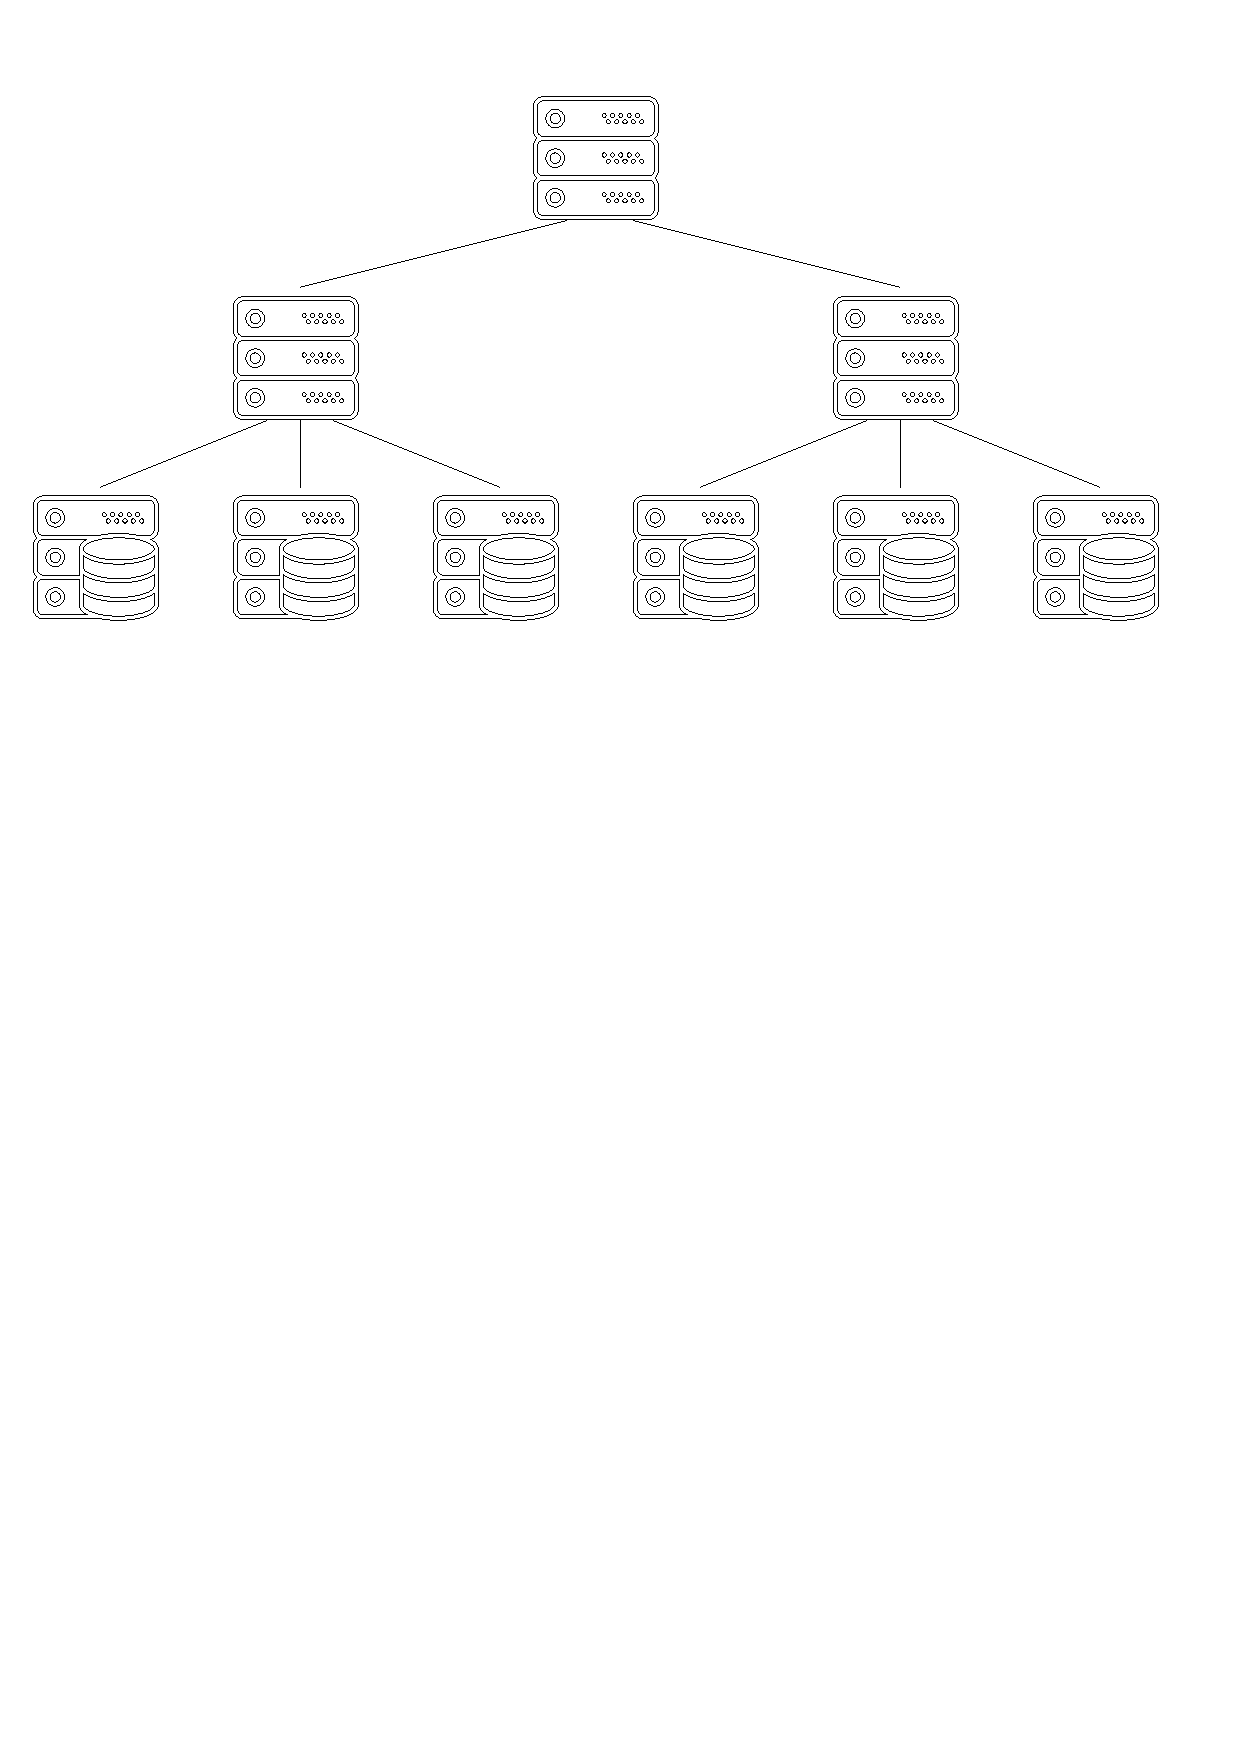
\includegraphics[width=0.79\columnwidth]{figs/tree-topology.pdf}
\caption{The model of typical data center with a tree-like network topology. We distinguish two types of tree nodes: the the intermediate nodes that transmit communication, and the computing machines, located at the leaves of a tree. Network links between nodes are depicted as solid lines.}\label{fig:tree-topology}
\vspace{-1em}
\end{figure}


\subsection{Our Contributions}

We consider two scenarios regarding virtual network embeddings:
\begin{enumerate}
  \item \emph{The static scenario}, where virtual machines are irrevocably assigned to their physical machines.
  \item \emph{The dynamic scenario}, where virtual machines can migrate between physical machines.
\end{enumerate}

We investigate the static scenario in Chapter~\ref{ch:static-mapping} and the dynamic scenario in Chapter~\ref{ch:dynamic-mapping}.
Although the problems are related by their practical motivations, their combinatorial structure differs substantially.
In particular, the static scenario is not an offline version of the problem considered in the dynamic one.
In both cases, we assume that the communication pattern among virtual nodes is not known in advance.
In the static scenario, we reserve a~portion of bandwidth between every pair of virtual nodes to allow for any possible communication pattern.
On~the~other hand, in the dynamic scenario, we react to changes in the communication pattern by migrating machines on the fly.
In addition, the problem considered in the static scenario is enriched to model the needs of batch-processing applications that use distributed file systems.


\subsubsection{Static Mapping of Virtual Networks}
\label{sec:contributions-static-mapping}

In the static scenario studied in Chapter~\ref{ch:static-mapping}, to guarantee a certain quality of service (\emph{QoS}), we acquire network reservations for all pairs of cooperating virtual machines.
The combinatorial problem that we consider in this scenario is essentially a variant of the minimum-cost embedding of~a~clique (the communication graph) in a tree (the substrate network).
In addition, the scenario is designed to model certain aspects of Map-Reduce~\cite{mapreduce}, which is a predominant framework for performing large-scale parallel data processing.
We consider the wide range of possible extensions that model certain aspects of Map-Reduce applications, most notably:

\begin{itemize}
\item \emph{Data chunk processing}. Virtual machines process large amo\-unts of data chunks that are stored in a distributed file system. Each chunk of data must be assigned to a virtual machine. Data chunk transfers require their own network reservations.

\item \emph{Data chunk replication}. Distributed file systems often store redundant copies of data chunks, called \emph{chunk replicas}. Only one copy of each data chunk replica must be processed, and we are free to choose the replica to be used based on its placement.

\item \emph{Bandwidth constraints}. Each link in the substrate network has its capacity. For the embedding to be feasible, the total network reservations have to obey link capacities.
\end{itemize}


We decompose the general optimization problem into its fundamental aspects, such as
assignment of chunks, replica selection, and flexible virtual machine
placement, and answer questions such as:
\begin{itemize}
\item How to efficiently embed virtual machines and their inter-connecting network?
\item Which data chunks to assign to which virtual machine?
\item How to exploit redundancy and select good data chunk replicas?
\end{itemize}

We draw a complete picture of the problem space: we show that
some problem variants (also those exhibiting multiple degrees of freedom in terms of
replica selection and embedding),
can be solved in polynomial time. For all other variants, we show limitations of their
computational tractability, by proving their NP-completeness. Interestingly,
our hardness results also hold in \emph{uncapacitated} substrate
networks of small-diameter networks (as they are
widely used today~\cite{fattree}).


\subsubsection{Dynamic Mapping of Virtual Networks}
\label{sec:contributions-dynamic-mapping}

In Chapter~\ref{ch:dynamic-mapping}, we study virtual network embeddings in the scenario where virtual machines can be migrated during runtime to another physical machine.
The possibility of migration allows reacting to unpredictable communication patterns.
For example, if some distant nodes communicate often, it is vital to reduce their distance to save network bandwidth.
The objective is to~minimize the total network bandwidth used for communication and for migration.

We assume that the communication patterns are not known in advance to our algorithm.
We measure the~quality of~presented algorithmic solutions by competitive analysis~\cite{borodin-book}, which is well-suited for problems that are online by their nature.
In the competitive analysis, the goal is to~optimize \emph{the competitive ratio} of a given online algorithm: the ratio of its cost to the cost of~an~optimal offline algorithm that knows the whole input sequence in advance.

In the dynamic scenario, we assume that the physical substrate network is a~tree of height one.
That is, every physical machine (leaf) is connected directly to the root (that has no hosting capabilities).
A single physical machine hosts a fixed number of virtual machines.
The model restricted to such networks becomes a variant of online graph clustering.
That is, we are given a~set of~$n$ nodes (virtual machines) with time-varying pairwise
communication patterns, which have to be partitioned into~$\ell$~physical machines, each of
capacity $k=n/\ell$.

Intuitively, we would like to minimize inter-machine
interactions by mapping frequently communicating nodes to the same physical machine
Since communication patterns change over time, the~nodes should be \emph{repartitioned}, in
an online manner, by \emph{migrating} them between physical machines.
The~objective is to minimize the weighted sum of inter-machine communication and repartitioning costs.
The former is defined as the number of communication requests between nodes placed at distinct physical machines, and the latter as the number of migrations.


The possibility to perform a migration uncovers algorithmic challenges:
\begin{itemize}

\item \emph{Serve remotely or migrate?} For a brief communication
pattern, it may not be worthwhile to collocate the nodes: the migration cost might
be too large in comparison to~communication costs.

\item \emph{Where to migrate, and what?}
If an algorithm decides to collocate nodes $x$ and~$y$, the~question becomes
how. Should $x$ be migrated to the physical machine holding $y$, $y$ to the one holding
$x$, or should both nodes be migrated to a new machine?

\item \emph{Which nodes to evict?}
The space of the desired destination physical machine may not be sufficient. In
this case, the~algorithm needs to decide which nodes to ``evict'' (migrate to
other machines), to free up space.

\end{itemize}

In the model described above, every physical machine fully utilizes its processing capabilities --- it hosts the maximum possible number of~virtual machines, i.e., $k=n/\ell$.
Hence, the migration is not possible without further reconfigurations: to respect physical machine capacity, we need to decide which virtual machines to swap.
For this setting, we show a deterministic lower bound of~$k$, where $k$ is the physical machines hosting capacity.
We also present a constant-competitive algorithm for the scenario restricted to physical machines that can host two virtual machines ($k = 2$).

In Chapter~\ref{ch:dynamic-mapping}, we also consider the resource-augmented scenario, where we relax the above assumption: now the total hosting capacity of physical machines exceeds the~total number of~virtual machines, i.e., $k > n/\ell$.
Surprisingly, the lower bound remains $k$ also in this setting.
The main contribution of this part is an $O(k\cdot \log k)$-competitive algorithm for the scenario with a small resource augmentation.

%This fundamental online optimization problem has many applications. For
%example, in the context of~cloud computing, $n$ may represent virtual machines
%or containers that are distributed across~$\ell$ physical servers, each having
%$k$ cores: each server can host $k$ virtual machines. We would like to
%(dynamically) distribute the virtual machines across the servers such that
%datacenter traffic and migration costs are minimized.


\subsection{Related Work}


Recently, there has been much interest in programming models and distributed
system architectures for processing and analysis of big data (see, e.g.,~\cite{mapreduce,nodb,shark}).
Such applications
generate large amounts of network traffic~\cite{orchestra,MogPop12,amazonbw},
and over the last years, several systems have been proposed that provide a provable network performance.
To guarantee a certain performance level, these systems reserve a portion of bandwidth among cooperating nodes.
There are two major approaches to bandwidth reservations: some systems depend on supplying the possibly different volume of bandwidth communication between each pair of nodes~\cite{faircloud,elasticswitch,seawall}, while other systems allocate abundant bandwidth of equal volume among all nodes~\cite{oktopus,secondnet,drl,gatekeeper,proteus}.
In this thesis we research both approaches: in Chapter~\ref{ch:static-mapping} we pre-reserve a portion of bandwidth among all cooperating nodes, while in Chapter~\ref{ch:dynamic-mapping} we perform the reservation as pairs of nodes communicate.

\medskip

In Chapter~\ref{ch:static-mapping}, we study virtual network embeddings, a problem of embedding a weighted \emph{guest} graph into a capacitated \emph{host} graph.
The virtual network embedding problem is related to~classic VPN graph embedding problems~\cite{gupta2001provisioning,vpn1, vpn2, Goyal2008},
a~problem that is NP-hard, and is constant-factor approximable even for asymmetric traffic demands~\cite{vpn-apx}.
The VPN problem requires finding a graph embedding with fixed endpoints, while in virtual network embedding problems, studied in this thesis, the embedding endpoints are also subject to optimization.
In this respect, the virtual network embedding problem can also be seen as related to
classic Minimum Linear Arrangement problem~\cite{EvNaRS99,ord-prob} which asks for the
embedding of communication graphs on simple line topologies.

We consider a variant of virtual network embedding with extensions motivated by batch-processing applications.
The most popular virtual network abstraction for batch-processing applications~\cite{mapreduce} is a virtual network that forms a clique~\cite{oktopus,MogPop12,infocom16,ccr15emb,proteus}.
Existing embedding algorithms often ignore a~crucial dimension of the problem, namely data locality:
an input to a batch-processing application is typically stored in a distributed
and sometimes redundant file system. Since moving
data is costly, an embedding algorithm should be aware of the data placement,
and allocate computational resources close to the data.
Redundant storage gives additional optimization possibilities.
In this thesis, we study data locality and replica-aware virtual network embeddings in tree topologies.
%Note that our variant is not strictly a~generalization of a virtual network embedding, as we took simplifying assumptions about the traffic demands.

\medskip

In Chapter~\ref{ch:dynamic-mapping}, we study an online balanced partitioning problem.
The static offline version of~the~problem, i.e., a problem variant where
migration is not allowed, where all requests are known in advance, and where
the goal is to find an assignment of $n$ nodes to $\ell$~physical machines, each of~capacity $n/\ell$, is known as the
\emph{$\ell$-balanced graph partitioning problem}. The problem is 
NP-complete, and cannot even be approximated within any finite factor unless P
= NP~\cite{AndRae06}.  The static
variant where $\ell = 2$ corresponds to the minimum bisection problem, which
is already NP-hard~\cite{GaJoSt76}, and 
the currently best approximation ratio is $O(\log n)$~\cite{SarVaz95,ArKaKa99,FeKrNi00,FeiKra02,KraFei06,Raec08}.
The inapproximability of the static variant for general values of $\ell$
motivated research on the bicriteria variant, which can be seen as the offline
counterpart of our capacity augmentation approach. Here, the~goal
is~to~compute a~graph partitioning into $\ell$ components of~size at most~$k$ (where $k > n/\ell$) and the cost of the cut is compared to the optimal (non-augmented)
solution where all components are of a~size at most $n/k$. The variant where
$n \geq 2 \cdot k \cdot \ell$ was considered in
\cite{LeMaTr90,SimTen97,EvNaRS00,EvNaRS99,KrNaSc09}. So far, the~best result~is~an~$O(\!\sqrt{\log n \cdot \log \ell})$-approximation algorithm~\cite{KrNaSc09}.

Our dynamic model is related to online
caching~\cite{SleTar85,FKLMSY91,McGSle91,AcChNo00}, sometimes also referred to
as online caching, where requests for data items (nodes) arrive over time and
need to be served from a cache of finite capacity, and where the number of
cache misses must be minimized. Classic problem variants usually boil down to
finding a smart eviction strategy, such as Least Recently Used (LRU)~\cite{SleTar85}. In our
setting, requests can be served remotely (i.e.,~without fetching the
corresponding nodes to a single physical machine). In this light, our model is more
reminiscent of caching models \emph{with
bypassing}~\cite{EpImLN11,EpImLN15,Irani02}. As a~side result, we show that our problem is
capable of emulating online caching.
A major difference between  these problems is that in the caching problems, each request involves a single element of the universe, while in our model \emph{both} endpoints of a communication request are subject to~optimization.



\section{Router Memory Optimization}
\label{sec:intro-packet-forwarding}


In the second part of this thesis, we consider the fundamental problem of \emph{packet forwarding}.
We focus on a single router, that physically connects different networks and is responsible for passing packets between them.
Upon receiving a data packet, the router forwards it to~a~specific output port leading to a neighboring network.
To choose an appropriate port, the router stores a~\emph{forwarding table}, which consists of rules describing how to map the packet destination addresses to appropriate ports.
Typically, a router stores a single rule for each network it knows about.

The router maintains the forwarding table in its memory.
Only a small restricted set of~operations is performed on such memory: lookups and updates.
Nowadays, routers perform millions of lookup operations and thousands of updates per second (see, e.g., a report~\cite{bgp-updates}), and use specialized hardware for the efficiency.
Hence, instead of using the general-purpose memory such as RAM, the specialized memory units such as TCAM are utilized~\cite{tcam-memory}.
The TCAM memory is associative memory storage that enables hardware supported pattern-matching lookup that closely matches the way the forwarding rules are used.

\subsection{Growth of Forwarding Tables}

Most routers located at the Internet core forward packets among a~large number of networks and have the knowledge about virtually all Internet networks.
Their forwarding tables are usually referred to as \emph{the global forwarding table} (Figure~\ref{fig:bgp-entries} depicts the growth of its size)~\cite{url-bgp-entries}.
Therefore, those routers have to store an~enormous number of forwarding rules: the
number of rules has doubled in the last six years~\cite{bgp-routeviews} and
the super-linear growth is likely to be sustained~\cite{steve-myth}.
It is worth noting that some of these networks are virtual.
The concept of virtual networks described in Part~\ref{pt:virtual-networks} contributed significantly to the partitioning of the Internet into subnetworks, and to further growth of forwarding tables.

In recent years, the size of forwarding tables started to exceed the amount of available TCAM memory in a typical router (the phenomenon called the TCAM exhaustion~\cite{tcam-exhaust}).
Sophisticated electronics circuits such as TCAM are very expensive and power-hungry in comparison to RAM~\cite{tcam-expensive}.
Moreover, typical operations performed on TCAM memory examine the whole contents stored in memory, which requires closely connected physical structure among memory cells --- as a result, available memory is expensive to expand.

The limited size of memory and expanding the size of the content to store brings new challenges in memory management of the routers.
In the second part of this thesis, we investigate the~following problem, using the tools provided by contemporary routers:
\begin{center}
  \emph{How to efficiently manage the memory of forwarding devices?}
\end{center}

\begin{figure}[t]
\centering
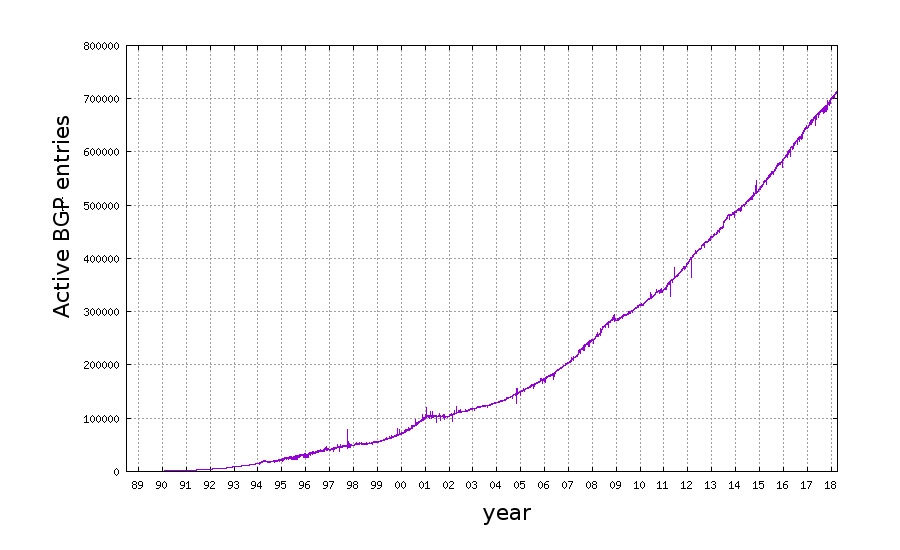
\includegraphics[width=0.79\columnwidth]{figs/bgp-entries.png}
\caption{The number of entries in the global forwarding table. The entries are built on the basis of informations exchanged via Border Gateway Protocol. The graph presents the growth of the global forwarding table from 1988 to 2018.}\label{fig:bgp-entries}
\end{figure}


\subsection{Our Contributions}

In Chapter~\ref{ch:packet-forwarding}, we study a novel solution for the management of a growing set of forwarding rules.
The idea that could delay the need for expensive or impossible memory upgrades in routers, is to store
only a subset of rules in the actual router and to store all rules on a~secondary
device (for example a commodity server with a large, but slow
memory)~\cite{cacheflow,route-caching-flat,prefix-caching,fib-caching-non-overlapping,fibium-zipf}.
%This solution is particularly attractive with the advent of Soft\-ware-Defined
%Network (SDN) technology, which allows to manage the expensive memory using a
%software controller~\cite{cacheflow,fibium-zipf}.
%In particular, our
%theoretical model can describe real-world architectures
%like~\cite{cacheflow,fibium-zipf},
%that is, our model formalizes the underlying operational
%problems of such architectures.
We propose a theoretical model for studying algorithmic solutions for such a setting.
This setting is similar to the caching problem: some rules are stored in a fast memory of~a~router.
We provide a natural online algorithm that dynamically manages the set of forwarding rules.
Our 
algorithm, when applied in the context of such architectures, can 
be used to prolong the lifetime of some routers.


%In this thesis, we investigate the scenario, where we store only the subset of forwarding rules in fast TCAM memory.
%If the forwarding rule is not present, we perform a query to slower (possibly remote) memory.
Although our theoretical model resembles the caching problem, the hierarchical structure of forwarding rules enforces some restrictions of cache configuration feasibility.
Forwarding rules form a~tree, and the child rule describes the exception to the parent rule.
To model this issue, we introduce a variant of caching, where the universe of elements (forwarding rules) form a~tree.
The child-parent relations express dependencies between cached elements: to preserve the semantics of the forwarding rules set, no parent rule can be in the cache without its child rules.
In other words, every valid cache configuration is a sub-forest.
We give a formal problem definition in Chapter~\ref{ch:packet-forwarding}.


We present a deterministic online algorithm for cache management with hierarchical dependencies, proving that it is
$O(h(T)\cdot k)$-competitive, where $h(T)$ is the height of the forwarding rules tree (the maximum nesting in the forwarding table), and $k$ is the size of the available cache.
Our result is optimal up to the factor~$O(h(T))$: we show that the lower
bound for the caching problem~\cite{SleTar85} implies an
$\Omega(k)$ lower bound for our problem.
While in theory $h(T)$ can be as large as the length of IP address, for the actual forwarding tables, it is a small constant (around 4--7).
In addition, we consider the online tree caching problem within the resource
augmentation paradigm: we assume that cache sizes of the online algorithm
($\kALG$)  and the optimal offline algorithm ($\kOPT$) may differ.
For this setting, we show that our algorithm is
$O(h(T) \cdot \kALG/(\kALG-\kOPT+1))$-competitive.


The performance of our algorithm is not degraded if the model is enhanced to handle rule updates (an important aspect of router operation).
Finally, we show that our algorithm can be implemented efficiently and without changes to the router software and hardware.

\subsection{Related Work}

We introduced a variant of caching with dependencies motivated by the structure of forwarding table.
In the framework of the competitive analysis, the caching problem was
first analyzed  by Sleator and Tarjan~\cite{SleTar85}, who presented $k$-competitive algorithms (where $k$ is the cache size) and a matching lower bound.
The problem was later generalized to allow different fetching
costs (weighted caching)~\cite{double-coverage,young-paging-greedy-dual} and
additionally different item sizes (file caching)~\cite{young-paging-landlord},
with the same competitive ratio.
%Asymptotically same results can be achieved
%when bypassing is allowed (see \cite{caching-rejection-penalties,paging-irani}
%and references therein).
%To the best of our knowledge, the variant of caching, where fetching items to
%the cache is not allowed unless some other items are cached (e.g., because of 
%tree dependencies) was 
%not considered previously in the framework of competitive analysis.


An important aspect of our problem is the dependency between forwarding rules.
So far, the papers on caching of forwarding tables avoided this issue, either assuming
that rules do not overlap (a~tree has a single level)~\cite{route-caching-flat} 
or by preprocessing the forwarding table, so that the rules become
non-overlapping~\cite{prefix-caching,fib-caching-non-overlapping}.
Unfortunately, this could lead to large inflation of the routing table. A
notable exception is a recent solution called CacheFlow~\cite{cacheflow}. The
CacheFlow model supports rule  dependencies even in the form of directed acyclic
graphs. However, CacheFlow was evaluated only experimentally, and no
worst-case guarantees were given on the overall cost of caching. Our work
provides theoretical foundations for respecting rule dependencies.


Other approaches for minimizing the number of stored rules were mostly based
on \emph{rules compression (aggregation)}, where the set of rules was replaced
by an another equivalent and smaller set. Optimal aggregation of a fixed routing
table can be achieved by dynamic
programming~\cite{ortc,fib-compression-two-dimensional}, but the main
challenge lies in balancing the achieved compression and the number of changes
to the routing table in the presence of updates to this table. While
many practical heuristics have been devised by the networking community for
this problem~\cite{mms,fib-compression-fifa,fib-compression-globecom10,fib-compression-infocom13,fib-sigcomm,fib-compression-smalta,fib-compression-infocom10},
worst-case analyses were presented only for some restricted
scenarios~\cite{fib-icdcs,fib-sirocco}. Finally, combining rules compression and rules
caching is so far an unexplored area.



\section{Bibliographic notes and acknowledgements}

The results of this thesis were published by its author in various conferences and journals.
Parts of Chapter~\ref{ch:static-mapping} appeared previously in the proceedings of~23rd~IEEE~International Conference~on~Network Protocols (ICNP~2015)~\cite{my-icnp}
and in Theoretical Computer Science, vol.~697~\cite{my-tcs}.
Some of the results from Chapter~\ref{ch:static-mapping} appeared in the Ph.D. thesis of my co-author Carlo Fuerst.
Parts of Chapter~\ref{ch:dynamic-mapping} appeared previously in the proceedings of~30th~International Symposium~on~Distributed Computing (DISC~2016)~\cite{my-disc}.
Chapter~\ref{ch:dynamic-mapping} contains a~thoroughly rewritten and improved revision of the results published in these proceedings.
Finally, parts of Chapter~\ref{ch:packet-forwarding} were published in the proceedings of~29th~ACM~Symposium on Parallelism in Algorithms and Architectures (SPAA~2017)~\cite{my-spaa}.
Some preliminary results from Chapter~\ref{ch:packet-forwarding} appeared in the master thesis of my co-author Aleksandra Spyra.

\medskip

This thesis was supported by the grant Preludium 2016/23/N/ST6/03412 for research on ``Online Algorithms for Packing and Covering Problems'' awarded by Polish National Science Centre.

